\documentclass[12pt, Times New Roman]{article}
\usepackage{mathptmx}

\usepackage{color}
\usepackage[dvipsnames]{xcolor}
\definecolor{darkblue}{RGB}{0.,0.,139.}

\usepackage[top=1in, bottom=1in, left=1in, right=1in]{geometry}

\usepackage{amsmath}
\usepackage{amstext}
\usepackage{amssymb}
\usepackage{setspace}
\usepackage{lipsum}

\usepackage{graphicx}
\graphicspath{ {images/} }

\usepackage{indentfirst}

\usepackage[authoryear]{natbib}
\usepackage{url}
\usepackage{booktabs}
\usepackage[flushleft]{threeparttable}
\usepackage{graphicx}
\usepackage[english]{babel}
\usepackage{pdflscape}
\usepackage[unicode=true,pdfusetitle,
 bookmarks=true,bookmarksnumbered=false,bookmarksopen=false,
 breaklinks=true,pdfborder={0 0 0},backref=false,
 colorlinks,citecolor=black,filecolor=black,
 linkcolor=black,urlcolor=black]
 {hyperref}
\usepackage[all]{hypcap} 
\usepackage{breakurl}   

\linespread{2}

\begin{document}

\begin{singlespace}
\title{ECON 5970 - Final Project \thanks{Thank you to Dr. Ransom, who is ever so helpful}}
\end{singlespace}

\author{Rachel Thatcher\thanks{Department of Economics, University of Oklahoma.\
E-mail~address:~\href{mailto:r.thatcher@ou.edu}{r.thatcher@ou.edu}}}

% \date{\today}
\date{April 26, 2018}

\maketitle

\begin{abstract}
\begin{singlespace}
This paper will cover how Twitter is being used by economists and how it is affecting their networks and the reach they are able to give their research. Specifically, it will focus in on citations and how they are related to the number of Twitter followers an economist has and the number of years they have been active. 

\end{singlespace}

\end{abstract}
\vfill{}


\pagebreak{}


\section*{Introduction}\label{sec:intro}
\setlength{\parindent}{10ex}


Since its creating in 2006 Twitter has grown rapidly to become one of the largest social media outlets on the face of the planet, with hundreds of millions of users logging on each month. While much of the content can safely be categorized as fairly inconsequential babble, there are a growing number of people who use Twitter for more academic purposes. Among them are many Economists, who have started taking to Twitter for more than just their own personal use. 

It is not an exaggeration to say how much of an impact social media is having on our lives, and so naturally more and more studies are coming out to see exactly what some of these impacts might be. One of these categories of research has focused on how, specifically, Twitter has been impacting the work of academics. As this rise of social media has only been really taking shape over the past decade or so and is thus still rather new and undefined, and there is still much more work to be done. But, seeing how social media only continues to grow around the globe, it seems likely that the research into this topic will continue to grow as well and this study hopes to add some small observations to it. 

This paper specifically focuses on some of the features of economists on Twitter, and look to see if there is a relationship between an economist’s popularity on Twitter and their success in the academic sphere. I first go over a review of the previous literature on the subject, most of which has been created around surveys and harvesting of tweets, and then moves on to the data I collected from the Research Papers in Economics (RePEc) website, which focuses more on the number and characteristics of those Economists who are on Twitter. Then a linear regression was used to see the relationship between the number of Twitter followers and the number of citations an Economist has, taking into account other relevant factors such as years active. The results showed a small relationship between having more followers and having more citations.



\section*{Literature Review}\label{sec:litreview}

With Twitter having been around for over a decade now there is an increasing number of studies being produced around its uses and possible roles in academia. Much of this work has been orchestrated through surveys and tweet collection, analyzing the words people use in their interactions on the site as well as the words they themselves use to describe it. For the purpose of these studies Twitter is almost always considered a ‘microblog’, or a social media sight which is used to make short and frequent posts \citet{Gerstein} .

Many of the studies coming out are looking at just what economists, and other academics, are using Twitter for. In \citet{Priem} they used both surveys with academics, focusing in specifically on how people cite on Twitter. They found that often Twitter is used for citation, but it is at a much faster rate than normal citation, with much of what is being shared having been published within merely a week or so. They also found that the citations are much more informal than they are in many other methods. One participant in the study described their Twitter feed as a “stream of lit review” as it would bring in constant new content to review and discuss. \citet{Priem} found that in this way Twitter was helping get information around the academic community quicker than previously, allowing users to build their network and reach places they may have not been able to with more traditional means. 

A similar result is found in a paper by \citet{Gruzd}, who also used surveys find what academics were using Twitter for. They found that academics were increasingly using Twitter to keep up with each other and work within the field in general, with it slowly starting to replace some older methods such as list serves and blogs for some academics. The participants stated that their main use of the site was to keep up to date with work in their field and find new works, and then to a lesser extent to network and promote their own work. They pointed to many scholars highlighting the speed at which they can review and find other’s work on Twitter, and how it can be used for information gathering and dissemination. Lastly, they found that Twitter is especially popular with academics during conferences, where it is preferred for the speed at which it can spread information relevant to what is going on at the conference and be used to keep up new networks and relationships that are being formed.

Another reason that academics are using Twitter is to build themselves a brand. While \citet{Priem} and \citet{Gruzd} saw academics building a network that allowed them to have a constant and up to date stream of new research in their field, other papers such as one by \citet{Budge} focus more on Twitter as a means for academics to network in the more active sense of the work, and get their own work and name out there by fostering more informal communication. They find that Twitter allows academics to foster relationships that they might not have been able to in real life, therefore breaking down in a way the older established forms of networking and communication within a community. They say that this could have potential benefits to more non-traditional academics, who now have greater accessibility and are more approachable online in a way that might help change the norms of academic discussion. 

A study by \citet{Staves} in 2012 reaches a similar conclusion, that many scholars are starting to use social media across the board to broaden their own horizons and get their research out there. They find that this trend is continuing to grow, and that more and more academic spheres are starting to outright incorporate social media into their system to help measure the success and impact research might be having at a more informal level. Beyond just getting their name out there to other academics, \citet{Staves} also finds that increasingly academics are using social media sites like Twitter to get their research out to the broader public as well.

However, when it comes to the specific use of Twitter to get information out to non-academics, many studies find that economists are behind the curve. In a recently unveiled paper \citet{Giusta} found that across the board scientists are better than economists at reaching the public. They are more informal with their speech and respond more to public inquires, while economists tweet less, use less accessible language, and interact less with the public. While this is a newer problem in concerns to social media, it is not a new problem in general. Academics, and specifically economists, have long seemed to the public to be a bit exclusive, using language and terms that are not accessible to those outside their fields. \citet{Giusta} study show that this problem seems to persist. 

In a similar vein of study \citet{Bahrani} found that this might be a larger trend for economists in general. Their paper looked at how technology as a whole is being incorporated into economic research and teaching methods alike and found that the discipline lags behind many of its peers. The paper suggests that Twitter and other social media sites can be helpful in the classroom if used properly, and that economists should try to catch up before they fall too far behind. 

Looking at all the literature together it paints the picture of economists using Twitter like many other people do, as an information stream, however theirs just happens to be academically focused. They use their feed to keep up to date with what is going on in their field and to explore various new papers and research as well as share articles and informal citations. Secondly, they use it network and build up a social brand, which some studies suggest could be a powerful tool in breaking down older communication structures and letting in voices that are not often heard. Lastly, the literature points to economists using Twitter to disseminate their own work, however it also shows that in many ways they may be lagging behind many of their academic peers in this regard. Going forward I think more research should be done into the networking aspect of it, to see if it really does increase the academic network of an economist. More specifically, I think it would be worth a look at the implications for minority demographics which are often left out of the traditional structures of communication. With less barriers to Twitter it could prove to help those who are often under represented, so it would be interesting to look into the demographics of those using Twitter to see if they lean more towards females or ethnic minorities than the population of economists as a whole

\section*{Data}\label{sec:data}

The data for this paper was collected from three different websites: the database of authors from the RePEc, the citations pages of these authors on Citations in Economics (CitEc), and the profiles of the authors on Twitter. I collected the first and last name and ID for every economist listed on RePEc, as well as their h index, i10 index, number of citations, and the number of years in which they have been active. The h index and i10 index are both used to see how influential each scholar has been holistically, with the h index measured as the largest number of papers an academic has published with h number of citations, and the i10 index was created by Google scholar and constitutes the number of papers an academic has that have been cited 10 times or more. In this way, both indexes inform the citation count and show the overall influence of an academic’s career, and make sure a person isn’t given a boost for one overall popular paper. The number of years is found by looking at the first year the author published a paper until now.  For those economists on Twitter I also collected their username, as well as the number of tweets they have created, the number of followers they have, and then number of accounts they are following. 

Overall, I ended up with 44,731 complete records of economists, of whom 1,101 were on Twitter. I chose these variables because this study aims to look at the relationship between Twitter usage and academic success for economists. The h index, citation count, and i10 index can all be used to measure the success of an economist, with the h index and citation count being the main two that will be looked at in this study. For Twitter popularity I used the number of followers a person had, as it shows their influence and the scope of their reach on the site. 

Looking at Table \ref{table1} we can see that for all economists on the site the mean h index is 5.168, while for economists who are not on Twitter, seen in Table \ref{table2}, it is slightly lower at 5.095 and for those on Twitter, Table \ref{table3}, it is higher at 8.056. The same pattern can be see for both the i10 index and the number of citations. All three of these categories skew right, as can be seen in Figure \ref{Hist1} and Figure \ref{Hist2} for the h index of both Twitter and non-Twitter economists. Economists who are not on Twitter have a lower mean than economists as a whole, and those on Twitter have a greater mean. This is also the case for median and standard deviation for all three of these categories. 

Just looking at these statistics it does appear that being on Twitter is correlated somewhat with greater success academically, with regards to a higher h index and i10 index, and more citations. However, we don’t know the cause of this. It could be that being on Twitter is helping economists gain more recognition and connections that result in a greater amount of citations, like many of the papers mentioned earlier suggest it might be. Or, it could just be that economists who would be more successful and active in promoting themselves academically anyway are the ones that then choose to get on Twitter. 
\newpage
One of the more interesting results I think is that the mean and median age for economists on Twitter is actually higher than that of those not on Twitter. And when you look at Figure \ref{Hist3} and Figure \ref{Hist4} you can see that there are relatively less economists on Twitter compared to non-Twitter economists. This is the opposite of what I assumed coming into the project as I suspected, and it was suggested by much of the previous literature, that those economists on Twitter would be younger, seeing as younger people tend to gravitate towards technology more and are in more need of promotion and networking.

\section*{Empirical Methods}\label{sec:methods}

Looking at the basic statistics for the data found that those economists who are on Twitter do seem to do better academically, wherein we define doing better academically as having a greater number of citations and higher indexes. So, now I will focus in on just those who are on Twitter, to see if there is a relationship between their popularity on Twitter and their academic success. To do this we will focus on the number of citations that an economist has, as both the h index and i10 index are derived from the number of citations and so covering citations in a way covers them as well. To measure popularity on Twitter we will look at how many followers an economist has. Lastly, we will also take into account how many years an economist has been active, as the longer they have been active the more time they have had to write papers and gather citations.
\newpage
We will run a regression on the data to see the relationship between citations, followers on Twitter, and years active. The formula we will use is:

\begin{equation}
log(Y) = \beta_0 + \beta_1x + \beta_2z + \beta_3z^2 + \epsilon
 \end{equation} 
where $Y$ is the dependent variable for citations, $x$ is the independent variable for the number of followers, $z$ is the independent variable for the number of years an economist has been active, and the parameter of interest is $\beta_1$.

\section*{Research Findings}\label{sec:results}

The results of our equation can be seen in Table \ref{table4}. The parameter of the number of followers an economist has is .217. And so, we can see that there is a positive relationship between the log of the number of citations an economist has and the number of followers they have. Meaning that if a person increases their followers on Twitter, they should see an increase in the number of citations they have, though possibly not a very large one. 

There is an even stronger relationship between the log of the number of citations and the number of years an economist has been active, a parameter of .256. This makes sense, as the longer an economist has been producing work the longer they have had for that work to be cited. However, it is interesting to see that the parameter for number of followers and number of years are actually very close to one another, showing that the relationship between citations and followers on Twitter might be stronger than one might initial expect. 

Looking at Figure \ref{Scat1} and Figure \ref{Scat2} we can see each of these relationships, between citations and followers and then between citations and years active, both play out through a simple linear regression. Both these graphs display what we already learned from Table \ref{table4}, that there is a positive relationship for both of the independent variables, but seeing them graphed separately shows us visually how years active is a bit steeper than followers.

These results further inform what several of the earlier studies discussed in the literature review were finding, if only through survey data. That is that having a Twitter can be a way of networking and getting oneself more exposure, which can lead to more academic success. 

\section*{Conclusion}\label{sec:conclusion}

Social media has spread to almost all parts of life it seems nowadays, and academia is no exception. Many academics see social medias such as Twitter as a way to connect to one another and keep up to date on what is going on in their field. Others see it as a way to build up their own recognition in the academic community and possibly beyond, using social media to spread the results of their studies with more ease. Most of what we know about how Twitter affects academics has been centered around surveys and examination of tweets. This paper relies on numbers scrapped from various economic websites and Twitter itself, using them to look at how followers and years of activity are related to the number of citations a person has. The analysis shows that there is in fact a positive relationship between both followers and citations, and years and citations, which makes a lot of sense. I would think further research into the topic could focus on looking at just exactly who is using Twitter or a closer look at its benefits with more variables in play than just years active. 

\vfill
\pagebreak{}
\begin{spacing}{1.0}
\bibliographystyle{jpe}
\bibliography{Final_Project.bib}
\addcontentsline{toc}{section}{References}
\end{spacing}

\vfill
\pagebreak{}
\clearpage

\section*{Tables and Figures}\label{sec:Tables and Figures}

\begin{table}[!htbp] \centering 
  \caption{All Economists} 
  \label{table1} 
\begin{tabular}{@{\extracolsep{5pt}}lcccccc} 
\\[-1.8ex]\hline 
\hline \\[-1.8ex] 
Statistic & \multicolumn{1}{c}{N} & \multicolumn{1}{c}{Mean} & \multicolumn{1}{c}{Median} & \multicolumn{1}{c}{St. Dev.} & \multicolumn{1}{c}{Min} & \multicolumn{1}{c}{Max} \\ 
\hline \\[-1.8ex] 
h.index & 44,731 & 5.168 & 3 & 5.713 & 0 & 90 \\ 
i10.index & 44,731 & 4.857 & 1 & 10.239 & 0 & 217 \\ 
citations & 44,731 & 282.942 & 43 & 1,051.376 & 0 & 48,387 \\ 
years.active & 44,731 & 12.612 & 10 & 10.177 & 1 & 57 \\ 
\hline \\[-1.8ex] 
\end{tabular} 
\end{table} 

\begin{table}[!htbp] \centering 
  \caption{Economists Not on Twitter} 
  \label{table2} 
\begin{tabular}{@{\extracolsep{5pt}}lcccccc} 
\\[-1.8ex]\hline 
\hline \\[-1.8ex] 
Statistic & \multicolumn{1}{c}{N} & \multicolumn{1}{c}{Mean} & \multicolumn{1}{c}{Median} & \multicolumn{1}{c}{St. Dev.} & \multicolumn{1}{c}{Min} & \multicolumn{1}{c}{Max} \\ 
\hline \\[-1.8ex] 
h.index & 43,630 & 5.095 & 3 & 5.549 & 0 & 90 \\ 
i10.index & 43,630 & 4.725 & 1 & 9.766 & 0 & 168 \\ 
citations & 43,630 & 270.144 & 42 & 961.458 & 0 & 48,387 \\ 
years.active & 43,630 & 12.562 & 10 & 10.190 & 1 & 57 \\ 
\hline \\[-1.8ex] 
\end{tabular} 
\end{table} 


\begin{table}[!htbp] \centering 
  \caption{Economists on Twitter} 
  \label{table3} 
\begin{tabular}{@{\extracolsep{5pt}}lcccccc} 
\\[-1.8ex]\hline 
\hline \\[-1.8ex] 
Statistic & \multicolumn{1}{c}{N} & \multicolumn{1}{c}{Mean} & \multicolumn{1}{c}{Median} & \multicolumn{1}{c}{St. Dev.} & \multicolumn{1}{c}{Min} & \multicolumn{1}{c}{Max} \\ 
\hline \\[-1.8ex] 
h.index & 1,101 & 8.056 & 5 & 9.863 & 1 & 87 \\ 
i10.index & 1,101 & 10.068 & 3 & 21.254 & 0 & 217 \\ 
citations & 1,101 & 789.147 & 101.5 & 2,830.858 & 1 & 34,823 \\ 
years.active & 1,101 & 14.340 & 13 & 9.515 & 1 & 57 \\ 
tweets & 1,101 & 5,338.851 & 1,354 & 362.390 & 1 & 176,000 \\ 
following & 1,101 & 697.195 & 392 & 1,191.812 & 0 & 14,900 \\ 
followers & 1,101 & 9,147 & 549 & 137,063.200 & 2 & 4,500,000 \\ 
\hline \\[-1.8ex] 
\end{tabular} 
\end{table}

\begin{table}[!htbp] \centering 
  \caption{Twitter Users: Regression} 
  \label{table4} 
\begin{tabular}{@{\extracolsep{5pt}}lc} 
\\[-1.8ex]\hline 
\hline \\[-1.8ex] 
 & \multicolumn{1}{c}{\textit{Dependent variable:}} \\ 
\cline{2-2} 
\\[-1.8ex] & log(citations) \\ 
\hline \\[-1.8ex] 
 log(followers) & 0.217$^{***}$ \\ 
  & (0.025) \\ 
  & \\ 
 years.active & 0.256$^{***}$ \\ 
  & (0.014) \\ 
  & \\ 
 I(years.active$\hat{\mkern6mu}$2) & $-$0.003$^{***}$ \\ 
  & (0.0004) \\ 
  & \\ 
 Constant & 0.330$^{*}$ \\ 
  & (0.188) \\ 
  & \\ 
\hline \\[-1.8ex] 
Observations & 1,101 \\ 
R$^{2}$ & 0.525 \\ 
Adjusted R$^{2}$ & 0.524 \\ 
Residual Std. Error & 1.489 (df = 1097) \\ 
F Statistic & 404.132$^{***}$ (df = 3; 1097) \\ 
\hline 
\hline \\[-1.8ex] 
\textit{Note:}  & \multicolumn{1}{r}{$^{*}$p$<$0.1; $^{**}$p$<$0.05; $^{***}$p$<$0.01} \\ 
\end{tabular} 
\end{table}

\begin{figure}[h]
    \includegraphics[width=.75\textwidth]{Histogram-Twitter-hindex.png}
    \centering
    \caption{Histogram of Twitter users looking at the frequency of their h indexes}
    \label{Hist1}
\end{figure}

\begin{figure}[h]
    \includegraphics[width=.75\textwidth]{Histogram-NonTwitter-hindex.png}
    \centering
    \caption{Histogram of non-Twitter users looking at the frequency of their h indexes}
    \label{Hist2}
\end{figure}

\begin{figure}[h]
    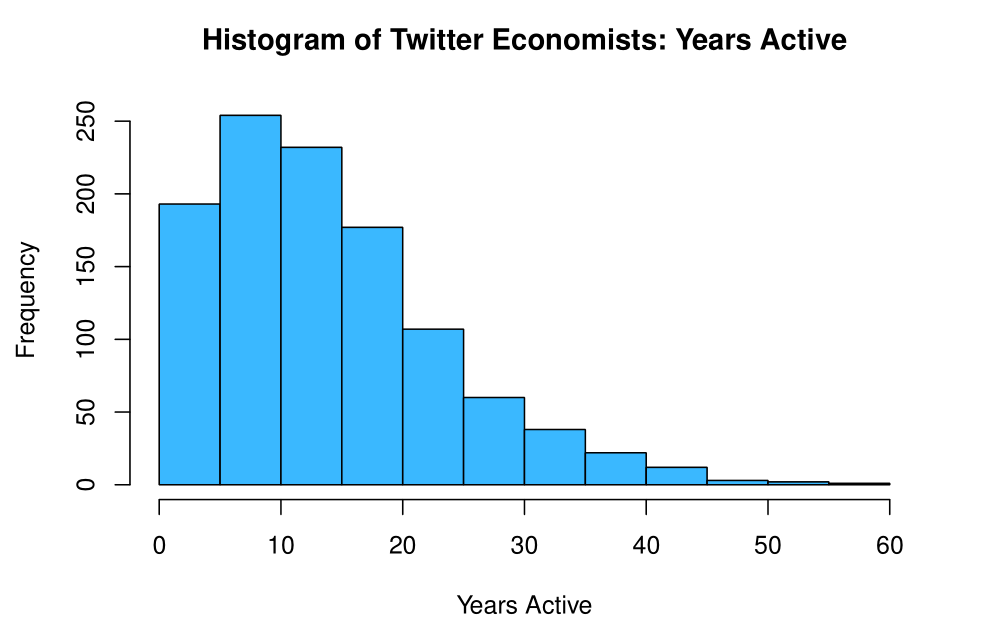
\includegraphics[width=.75\textwidth]{Histogram-Twitter-yearsactive.png}
    \centering
    \caption{Histogram of Twitter users looking at the frequency of their years active}
    \label{Hist3}
\end{figure}

\begin{figure}[h]
    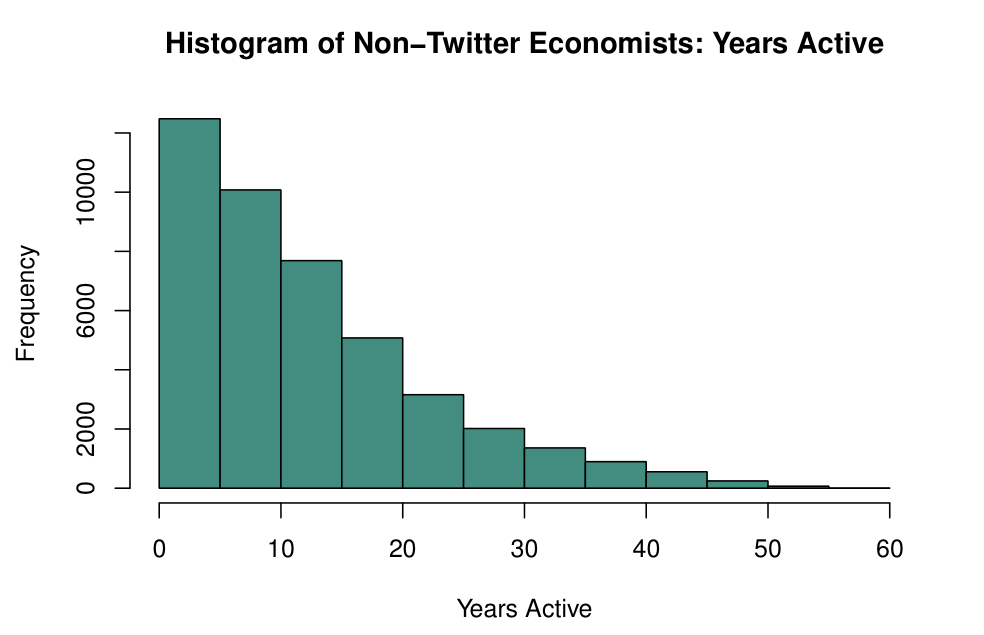
\includegraphics[width=.75\textwidth]{Histogram-NonTwitter-yearsactive.png}
    \centering
    \caption{Histogram of non-Twitter users looking at the frequency of their year active}
    \label{Hist4}
\end{figure}

\begin{figure}[h]
    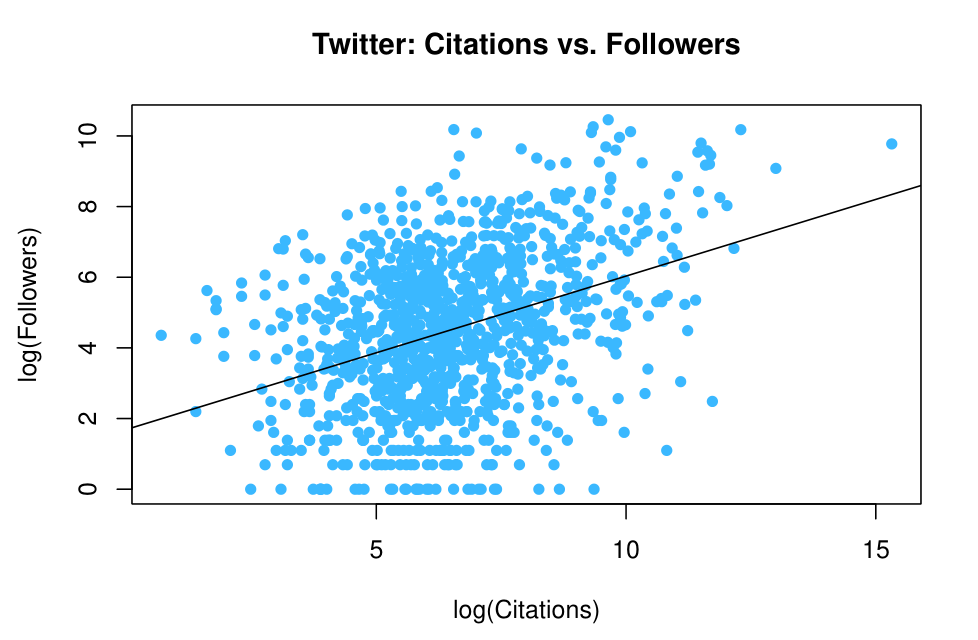
\includegraphics[width=.75\textwidth]{Scatter-Followers.png}
    \centering
    \caption{Linear regression and scatter plot of Twitter users' log of citations with regard to the log of their number of followers}
    \label{Scat1}
\end{figure}

\begin{figure}[h]
    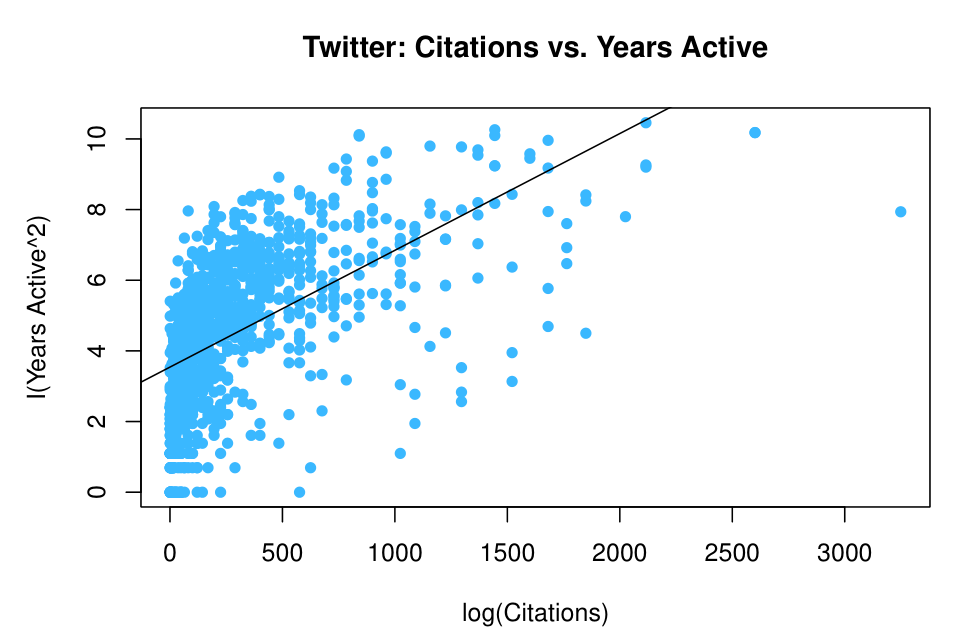
\includegraphics[width=.75\textwidth]{Scatter-YearsActive.png}
    \centering
    \caption{Linear regression and scatter plot of Twitter users' log of citations with regard to their number of years active squared}
    \label{Scat2}
\end{figure}

\end{document}}
